\section{Introduction}
In this section we provide a review of the literature relevant to our
current and planned research. We begin with a review of simultaneous
localisations and mapping (SLAM) systems, which is relevant because the
research presented in the remainder of this report involves reasoning
processes that utilise SLAM systems to provide known camera
poses.

We then turn to a review of the use of context in robotics
applications, a subject that has received somewhat sparse attention in
the literature and has, as yet, no cohesive formulation or problem
statement. Following this we examine the more detailed literature on
context in computer vision. This area is of great interest since many
of the techniques may be transferable to our setting.

\section{SLAM}
In order for a robot to navigate within an unknown environment it must
build a map of its environment and simultaneously localise itself
within that map. The representation of the map and robot pose, and the
techniques used to estimate these quantities, form the problem known
as simultaneous localisation and mapping (SLAM). These problems are
difficult because the solution to either part seems to rely upon the
solution to the other in a chicken--and--egg--style regression, yet it
is also a problem of great importance, since a working SLAM system is
a first requirement for many robotics and vision tasks, such as
navigation, path planning, spatial reasoning, and augmented reality.

Despite the considerable progress of SLAM systems over the past two
decades, they are still imperfect and cannot be treated as infallible
black boxes --- some understanding of the issues involved is
necessary. However, our work is intended to \textit{utilise} SLAM
rather than improve upon the state--of--the--art so we keep this
section brief, simply outlining the major paradigms within the
literature.

\subsection{Extended Kalman Filter}
The Kalman filter \cite{Kalman60} is a recursive state estimator that
has been applied to a diverse range of problems. SLAM can be posed as
an estimation problem is which the system state comprises both the
robot's location and the 3D location of landmarks in the
environment. The Kalman filter cannot be directly applied here because
it assumes a linear relationship between sensor inputs and the
underlying system state, which almost never holds true for the SLAM
problem. The Extended Kalman Filter (EKF) is a generalisation that can
deal with nonlinear functions by approximating them as piecewise
linear. Smith and Cheeseman were the first to apply the EKF to SLAM
\cite{Smith87}.

The EKF has two drawbacks worth mentioning here. First, it maintains a
full covariance matrix over the system state, which in the case of
SLAM grows with the number of landmarks. This covariance matrix must
be updated at each step, which requires $O(n^2)$ time for $n$
landmarks, so the computational cost grows quickly as the map expands.

Second, the EKF assumes that all measurements and state estimates have
Gaussian--distributed errors. While this is a reasonable
characterisation of the sensors themselves, the observations in each
frame must be associated with landmarks from the map and if there is
significant uncertainty about this data--association then the overall
error distribution is highly non--Gaussian.

Montemerlo \etal \cite{Montemerlo02} have proposed a system known as
FastSLAM to try to overcome some of these problems. FastSLAM maintains
a particle filter over robot poses, with each particle maintaining a
separate EKF over landmark locations.

\subsection{Parallel Tracking and Mapping}
An alternative approach to SLAM comes out of the extensive work on
structure from motion in computer vision, where the reconstruction of
camera poses and 3D landmark positions is approached as a single
``after the fact'' estimation problem \cite{Hartley04}. Within this
setting the dominant approach is to incrementally adjust both the pose
parameters and landmark locations by gradient descent methods. In the
literature this is known as bundle adjustment, but while it is highly
accurate, it is also too computationally intensive to run on--line for
every frame in a video sequence.

Klein and Murray \cite{Klein07} have proposed to overcome this by
running bundle adjustment periodically for a small set of keyframes
sampled from the video stream. Their system, called parallel tracking
and mapping (PTAM), uses this bundle adjustment to resolve the 3D
locations of a set of landmarks, which are then tracked through the
remainder of the video stream. As new frames arrive, the tracker
identifies known landmarks and computes the camera pose using the
known 3D locations of the landmarks. During this process the landmarks
are considered fixed, so only the camera pose is being estimated,
which makes this a very efficient operation.

When the system deems it necessary, an incoming frame is selected to
become a new keyframe, which adds a new set of landmarks to the
map. The bundle adjuster then sets to work updating the position of
all landmark locations and camera poses in a separate thread, while
the landmarks continue to be tracked in real--time. On modern
multi--core CPUs this allows the tracker to maintain video--rate
performance whilst the map is being periodically updated in the
background. An example frame from PTAM is shown in
\figref{klein-result}.

PTAM possesses a number of advantages over other SLAM systems. First,
the separation of tracking and mapping into separate threads allows
PTAM to maintain very dense maps (thousands of points), which would be
intractable for real--time performance under other SLAM paradigms.
Second, PTAM is robust to measurement errors because frames containing
poor measurements will not be selected for incorporation into the
map. PTAM also gains robustness from the large number of landmarks it
tracks, which allows a robust estimator to reliably find a subset of
inliers even when many measurements constitute outliers.

\begin{figure}[htp]
\centering
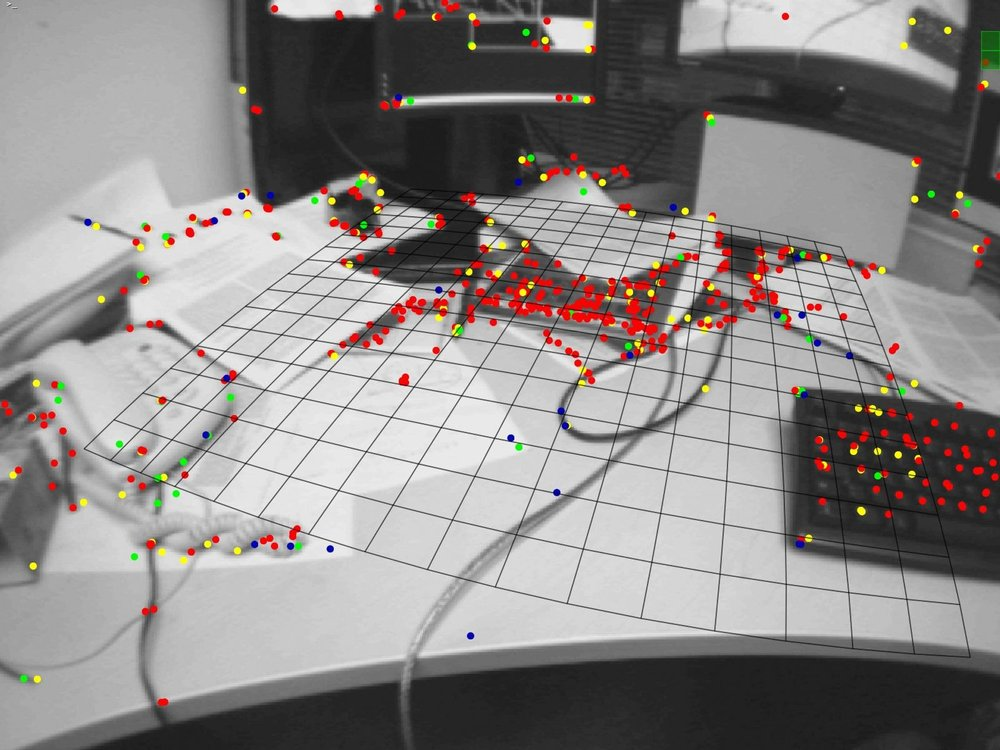
\includegraphics[width=0.6\textwidth]{klein_result.jpg}
\caption{A set of landmarks features identified by the PTAM system of
  \cite{Klein07}. The grid shows the dominant plane for the 3D point
  cloud and the colours indicate the system's confidence in landmark
  localisation.}
\label{fig:klein-result}
\end{figure}

\section{Context in Robotics}
Cameras have long been recognised as a valuable sensor for mobile
robotics. In addition to visual SLAM, cameras have been used in
robotics tasks such as place recognition \cite{Cummins08} and scene
description \cite{Posner08}. Contextual reasoning, in which
observations are understood in terms of their relationship to ``the
bigger picture'', has received little attention from the robotics
community. This section reviews the literature that does exist on this
topic. We divide the work into two categories: robo--centric
approaches, which organise sensor data as a time--indexed series of
observations, and map--centric approaches, which integrate sensor data
into a map and then reason from this representation.

\subsection{Robo--centric approaches}
Martinez \etal \cite{Mozos05} have demonstrated that a robot can learn
to classify its environment into semantic categories such as
``corridor'' or ``room'' based on simple range data features. They
employ a SICK laser, which gives a $360\degrees$ scan of the scene
within a single horizontal plane. They collect features such as the
distance between successive beams, the average beam length, and the
eigenvalues of the polygon formed by the beam endpoints, which are
concatenated to form a feature vector at each time step.

To relate these features to semantic categories, the authors employ
the AdaBoost algorithm \cite{Schapire98} using linear classifiers as
the weak learners. AdaBoost is a popular classifier that learns by
incrementally adding rules that maximally correct the mistakes it has
made so far. Martinez \etal show that they are able to differentiate
rooms, corridors, and doorways at up to 89\% accuracy using this
method. Furthermore, in environments that have not been seen before
the system obtains 82\% accuracy. The results for one environment are
depicted in \figref{martinez-result}.\\

\begin{figure}[htp]
\centering
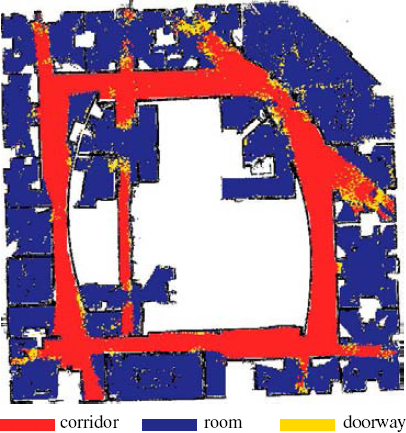
\includegraphics[width=0.5\textwidth]{martinez_result.png}
\caption{Semantic labels assigned by the range data classification
  system of Martinez \etal \cite{Mozos05}. 82\% of places were
  correctly classified, despite the environment not having been seen
  during training.}
\label{fig:martinez-result}
\end{figure}

Stachniss \etal \cite{Stachniss05} extends this to use visual cues
from a panoramic camera in addition to the laser range data. Stachniss
runs an off--the--shelf object detector for each of several object
categories that correlate well with location. The chosen objects
include computer monitors, coffee machines, and soap dispensers. At
each time step, the robot's current location is categorised using the
same AdaBoost classifier as described above, the only difference being
that now the number of visual detections of each object type are
appended to the AdaBoost input vector. This allows the classifier to
select between visual and range data features (or combinations
thereof) according to whichever is most salient for the task at hand.

The authors recognise that the robot's location is highly correlated
over successive time steps and so model the robot's state as a Hidden
Markov Model (HMM), with the transition probabilities estimated
empirically. Stachniss \etal show that the addition of visual cues
allow them to differentiate between rooms with a similar shape but
different visual appearance (such as bedrooms and living rooms),
whereas the original range--data--only approach of Martinez would fail
in this case.\\

Posner \etal \cite{Posner08} show how to learn semantic labels such as
``grass'', ``foliage'', or ``wall'' for regions within urban
environments. Like the systems described above, they reason from a
combination of laser and vision features, including colour, location,
and orientation properties. Unlike previous approaches they perform a
quantisation step to form feature ``words''.

Incoming images are segmented based jointly on an off--the--shelf
superpixel algorithm and continuity boundaries in the laser data,
after which the problem is reduced to determining the appropriate
label for each segment. They relate the features for each region to
semantic labels using a graphical model that incorporates observation
likelihoods as well as a sensor model describing the probability of
false positive and false negative observations. While a standard
approach would be to assume independence between the feature
observations for tractability, the authors note that the observations
are far from independent in reality and instead employ the Chow Liu
algorithm to find the best tree--structured approximation to the full
joint distribution. Inference within this model is performed by
computing the full posterior over labels.

Posner \etal further refine the labelling by relating the labels of
neighbouring patches in an MRF framework. They introduce edges for
both spatial and temporal consistency, the former being derived from
adjacency between segments within the image, and the latter being
derived by reprojecting laser points into consecutive frames. Node
potentials are given by the segment classifier described above
while edge potentials are learned empirically from hand--labelled
training data. Sequential tree--reweighted message passing (TRW--S) is
chosen for inference within the MRF due to its efficiency guarantees.

The authors show that their system is able to accurately label a range
of outdoor environments with 8 categories (grass, tarmac, dirt path,
textured wall, smooth wall, foliage, vehicle). Their classifier
obtains the highest precision for the ``grass'' category ($95.5\%$)
and the lowest for ``vehicles'' ($79.7\%$). Furthermore, their system
is able to run in under 4 seconds, which is suitable for periodic
on--line operation. An example labelling is illustrated in
\figref{posner-result}.

\begin{figure}[htp]
\centering
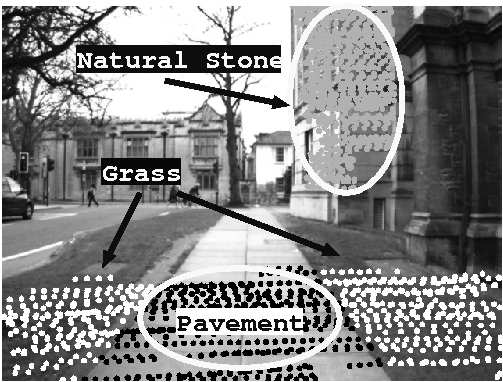
\includegraphics[width=0.8\textwidth]{posner_result.png}
\caption{Semantic labels output by the system of Posner et al
  \cite{Posner08}.}
\label{fig:posner-result}
\end{figure}

\subsection{Map--centric approaches}
An alternative approach to deriving context in robotics applications is
to integrate new measurements into a map, and then reason about
semantics within the map representation. In general this approach
enables stronger integration of measurements taken over several time
steps, at the cost of relying on the ability to correctly build a map.

Buschka and Saffiotti \cite{Buschka02} have taken a map--centric
approach to the problem of identifying room boundaries within indoor
environments and recognising the resultant rooms. A series of laser
range scans are fused into a 2D occupancy grid representing the
probability that each cell is occupied by some object or
boundary. Rooms boundaries are identified by applying dilation and
erosion to the occupancy map, which are standard morphological filters
from visual segmentation \cite{Forsyth02}. The
authors demonstrate that this can be performed with fixed
computational cost by discarding old parts of the environment as the
robot moves through the environment.

The result of their algorithm is a series of ``nodes'' with topological
connections between them, which correspond to the various rooms and
corridors within the robot's environment and the doorways that connect
them. The authors proceed to characterise each node by the size and
eccentricity (length to breadth ratio) of its bounding box. This gives
contextual information in two senses: firstly, the identification of
room boundaries allows reasoning in terms of rooms rather than the
entire known environment, and secondly, the characterisation of room
shapes allows differentiation between rooms and corridors and thus
allows different interpretations of sensor data in these semantically
distinct workspaces.

Vasudevan \etal \cite{Vasudevan07} use an alternative map representation
based around the location of objects. They argue that this matches
human perception of space. In their maps, each ``object'' (actually a
SIFT landmark) occupies a separate coordinate frame, with uncertainty
represented in the transformations between frames.

They identify doorways by running a line detector and testing various
combinations of lines against a set of heuristics, enabling separation
of the constituent rooms within an environment. This in turn allows
per--room reasoning as was the case with the Buschka and Saffiotti
system described above. The difference here is that Vasudevan \etal
identify doorways directly from visual input whereas Buschka and
Saffiotti use occupancy maps.

Vasudevan \etal show that this representation leads naturally to
reasoning about place context. They argue that place categories
(bedrooms, kitchens, bathrooms, \etc) can be identified by the objects
within them, and hence that their object--centric maps provide the
perfect setting for this form of contextual reasoning. Formally, they
learn a class--conditional object likelihood by computing the number
of times each object is observed in each type of places versus the
total number of times the place category has been observed. They then
assume independence between object observations and compute the
posterior over place categories by multiplying out the likelihoods for
each observed object. An example map and the robot's inferences about
place categories is shown in \figref{vasudevan-result}.

\begin{figure}[htp]
\centering
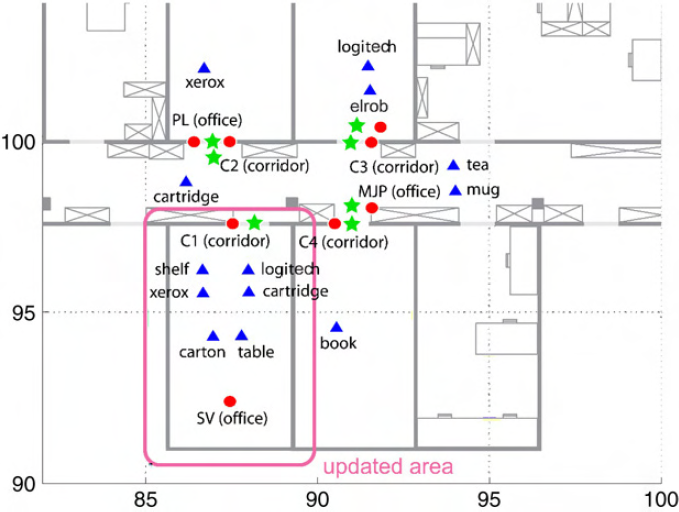
\includegraphics[width=0.75\textwidth]{vasudevan_result.png}
\caption{Example of an object--centric map of \cite{Vasudevan07}. The
  blue triangles show object detections, the red and green stars show
  doorways the system has identified, and the red dot shows the
  robot's inferred place category for the outlined room, which in this
  case is an office.}
\label{fig:vasudevan-result}
\end{figure}






\section{Context in Computer Vision}
Over the past decade there has been renewed interest in the use of
contextual information for computer vision tasks. There is a plethora
of definitions of what ``context'' means and how to represent it. Here
we review the dominant paradigms that have emerged around contextual
reasoning in single image understanding. Many of the single--image
contextual approaches have been targeted at a specific problem ---
namely that of object recognition --- and while this is not aligned
exactly with our own goal it is still instructive to review these
contributions because the ideas they propose for inferring context are
often separable from the specific task on which the authors choose to
demonstrate them.

\subsection{Holistic Approaches}

\subsubsection{Gist Features}
The work of Torralba \etal \cite{Torralba03} has been very influential
in expounding the value of contextual reasoning for vision. In their
work, they compute a feature vector composed of statistics from the
entire image and use this to reason about the contents of the
image. This feature vector is termed the ``gist'' of the image and is
computed as follows. First, an input image is passed through a bank of
Gabor filters at $n$ orientations and $m$ scales, producing $nm$
response images. Next, each response image is divided into a $k \times
k$ grid. Finally the average over each grid cell is computed for each
response image, and these values are concatenated to form the final
feature vector of length $nmk^2$.

In early work, Torralba \etal used the gist vector to learn about
scene categories. They showed that images could be classified into
categories such as ``road'', ``forest'', and ``bedroom'' by applying a
support vector machine (explained below) directly to the gist
vector. In later work \cite{Torralba03} they show how the location and
scale of objects can be predicted from the gist vector. The
Expectation--Maximisation algorithm \cite{Dempster77} is employed
to learn a mixture of Gaussians that relates the gist features to the
probability of an object being present at various locations and
scales. An example prediction is shown in \figref{contextual-priming}.

Support vector machines (SVM) were proposed by Vapnik \cite{Vapnik95}
just over a decade ago and have since gained widespread support both
inside and outside the machine learning community. SVMs learn to
discriminate two classes by finding the separating hyperplane in
feature space for which the distance to training examples is
maximised.

The Expectation--Maximisation algorithm is a widely used tool for
parameter estimation in the presence of unobserved variables
\cite{Dempster77}. Direct inference in such cases would require
marginalisation over all unobserved variables, but the integrals
involved typically make this approach infeasible. The EM algorithm
overcomes this by iterating between two stages. First, the expected
likelihood is computed with respect to the unobserved variables (the
E--step), and second, the model parameters are maximised with respect
to the distribution computed in the first step (the M--step). These
steps are repeated until convergence.

\begin{figure}[htp]
\centering
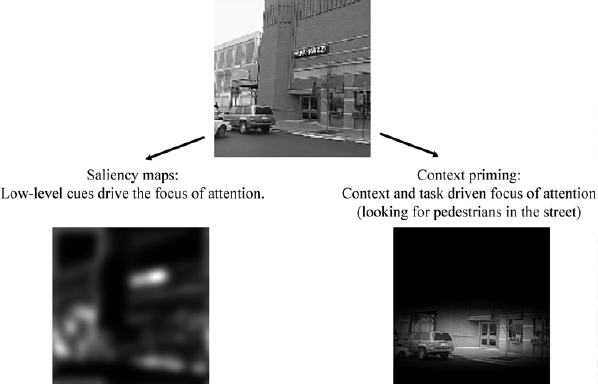
\includegraphics[width=0.75\textwidth]{contextual_priming.png}
\caption{Torralba's system \cite{Torralba03} is able to improve upon
  traditional interest point detectors by learning the relationship
  between gist features and probable object locations. Image taken from
  \cite{Torralba03}.}
\label{fig:contextual-priming}
\end{figure}

\subsubsection{Semantic Scene Labels}

Fei--Fei and Perona \cite{Fei-fei05} have proposed to classify images
explicitly into semantic categories such as ``coastal'', ``inner
city'', or ``bedroom''. Although their work focuses on the
classification task itself, the output scene label is clearly a useful
piece of contextual information for integration into a broader scene
understanding system.

Fei--Fei and Perona represent an image as a bag of words, where the
``words'' are obtained by clustering SIFT features (explained below)
obtained at regularly sampled locations across all training
images. Once the codebook of words has been learnt, each image is
collapsed to a simple sequence of integers representing the index of
the codebook entries identified within it.

Analogous to document understanding approaches in which each section
is associated with an inferred topic, Fei--Fei and Perona model a
hidden ``topic'' variable for each image feature. In their model they
also include a theme variable, which induces a class--conditional
multinomial distribution over topics.

On a dataset of 15 scene categories, each with several hundred images
taken from the web as well as from datasets released by other
researchers, the system obtains an average classification accuracy of
$64.0\%$.

The scale--invariant feature transform (SIFT) was first proposed by
Lowe \cite{Lowe99} for use in object recognition. Given some input
image, SIFT generates a set of interest points and corresponding
feature vectors that are robust to changes in lighting, scale, and
camera viewpoint. To select salient features at a range of sizes, SIFT
builds a scale--space representation of the image \cite{Lindeberg93}
and selects locations that are well--localised in both the spatial and
scale dimensions. Features are generated from a histogram over
gradient orientations in a patch around each selected interest
point. SIFT is now used for many tasks throughout computer vision.

\begin{figure}[htp]
\centering
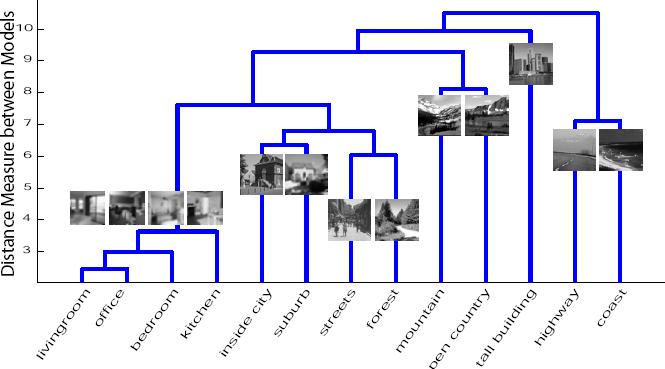
\includegraphics[width=\textwidth]{feifei_dendogram.png}
\caption{Dendogram showing the relationships between scene categories
  learnt by the system of Fei--Fei and Perona \cite{Fei-fei05}. The
  model matches human intuition well. Image taken from
  \cite{Fei-fei05}.}
\label{fig:dendogram}
\end{figure}

\subsection{Geometric Approaches}

An explicit understanding of scene geometry can assist image
understanding in numerous ways. Several authors have shown how to
obtain coarse 3D reconstructions from a single image, which allows
rich geometric reasoning for inference about such things as the
objects and actions likely to occur within the scene, and the scale
and position at which these might be found.

\subsubsection{Pixel--wise Geometry Estimates}

Hoiem \etal \cite{Hoiem06} approach geometric context as a per--pixel
labelling problem in which the labels identify geometric properties of
the 3D surface from which each pixel was captured. Although there are
many 3D scenes that could have generated any particular image, Hoiem
\etal note that some scenes are more probable than others given our
knowledge of the world. To keep this difficult inference task
tractable, the authors limit the pixel labels to ``sky'', ``ground'',
and ``vertical'', the last of which is further sub--divided into
``left--facing, ``right--facing'', and ``front--facing''. While there
are some real--world scenes that cannot be represented by these
geometric primitives, the authors show that they are able to model
many useful and interesting types of scenes.

The authors take a machine learning approach to the reconstruction
problem. First, the image is over segmented into superpixels using the
algorithm of Felzenszwalb \etal \cite{Felzenszwalb04}. Next, pairs of
adjacent superpixels are merged in order to gradually grow the small
superpixels into larger regions. To do this, an affinity metric
between adjacent superpixels is learnt using a boosted decision tree
classifier, the input to which is a feature vector containing cues
such as colour, texture, location, shape, and vanishing points. At
evaluation time many different segmentations are generated by
considering the superpixels in different orders. For each ordering,
the first $k$ superpixels are assigned to unique segments, then the
remaining superpixels are assigned to the segment with which they have
the greatest affinity. Each segment is classified into one of the
geometric classes listed above using another a boosted decision tree
classifier with the same input cues as for the affinity metric
learning. Finally, superpixels are labelled according to the consensus
vote amongst the segments to which they belong.

The authors further show that the geometric labels obtained in this
way can be used as priors for object detection, since detections in
unlikely places and scales can be suppressed, while those in
geometrically consistent positions can be
amplified. \figref{hoiem-result} shows the improvement in detection
performance resulting from the use of geometric context.

\begin{figure}[htp]
\centering
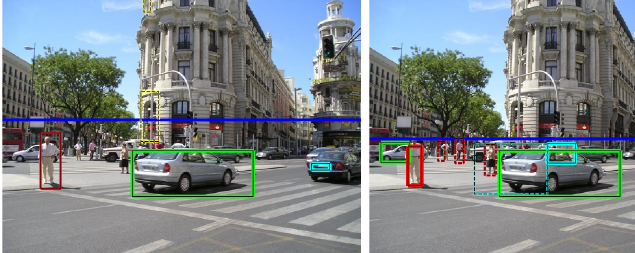
\includegraphics[width=\textwidth]{hoiem_detection_result.png}
\caption{The left image shows car and pedestrian detections when using
  local features only. The right image shows detections when geometric
  context is leveraged: several false--positives are eliminated and
  several new correct detections are made. Image taken from
  \cite{Hoiem06}.}
\label{fig:hoiem-result}
\end{figure}

\subsubsection{Make3D}

Another approach to deriving geometric context has been proposed by
Saxena \etal \cite{Saxena09}. Rather than the fixed set of
orientations employed by Hoiem \etal, Saxena \etal only assume that
the scene is piece--wise planar. They allow these planar patchlets to
take on arbitrary orientations, which they represent with a normal
vector.

Simpler to Hoiem's approach, Saxena \etal apply a machine learning
methodology to this problem. They begin by dividing the image into
superpixels, each of which is associated with a feature vector
containing the output of a set of filters, including colour, texture,
and edges. Each superpixel also includes the features of neighbouring
superpixels so that the inference process can reason in terms of
broader image properties rather than local statistics alone. In
addition, each superpixel boundary is associated with a separate set
of features. These are generated by running segmentations based on
different image properties and recording whether the boundary is
present in each.

The superpixels are organised into a Markov Random Field (MRF), with
edges between pairs that share a boundary in the image. The node
potentials are learnt from the superpixel features and edge
potentials are learnt from the boundary features. The authors allow
for coplanar, connected, and disconnected relationships across
boundaries, with the former preferred \textit{a priori} over the
latter. The MRF parameters are learnt through Multi--Conditional
Learning and inference is performed by solving a linear program.

Within a dataset of 152 internet images the system was able to
generate a qualitatively correct model (as judged by a human) 64.9\%
of the time. One such result is illustrated in \figref{saxena-result}.

\begin{figure}[htp]
\centering
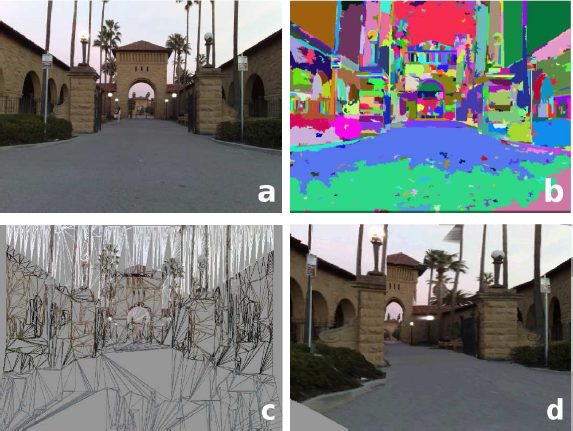
\includegraphics[width=0.5\textwidth]{saxena_results.png}
\caption{Results from the geometric context system of Saxena \etal
  \cite{Saxena09}. From top left to bottom right the panes show (a)
  the original, (b) the superpixels, (c) the inferred 3D model, (d) a
  re--projection of the 3D scene.}
\label{fig:saxena-result}
\end{figure}

\subsubsection{Manhattan World Models}

Lee \etal \cite{Lee09} have investigated geometric context for the
special case of indoor environments. By restricting themselves to a
particular class of scenes they can make use of more detailed prior
knowledge. They make the following assumptions about indoor scenes:
\begin{itemize}
  \item{There is a floor plane and a ceiling plane, which are parallel
    to one another and extend indefinitely in all directions.}
  \item{There are planar wall sections, which are orthogonal to the
    floor, extend all the way from the floor to the ceiling, and
    terminate in vertical boundaries.}
  \item{The wall sections are oriented in one of two mutually
    orthogonal directions.}
  \item{Many objects within rooms are aligned with the floor and/or
    walls and hence there will be many edges sharing vanishing points
    with floor, walls, and ceiling.}
\end{itemize}

Although there do exist exceptions to these rules, the authors argue
that a broad enough class of scenes is covered to justify their
choice. The authors thus adopt the Manhattan world assumption of
Coughlan and Yuille \cite{Coughlan99}, in which the world is built in a
Manhattan grid structure. For indoor scenes this leads to a
particularly simple model in which scenes are represented by a ground
plane orientation and a set of wall segments.

Lee \etal show how such a model can be derived from a single
image. They begin by sampling two pairs of lines in a RANSAC--like
fashion to generate vanishing points. Each pair is checked for mutual
orthogonality (using a prior on camera focal length) and for support
amongst the other detected line segments. The intersection of the two
pairs gives two vanishing points, from which the third can be
derived. This results in a set of straight lines and their associated
vanishing points.

The authors show that, given the assumptions above, any set of lines
representing wall segments for which the associated vanishing points
are known either give rise to exactly one Manhattan world model or
violate a set of easily--checkable rules. They therefore proceed to
enumerate all valid hypotheses by running a branch--and--bound search
over all combinations of line segments. This remains tractable because
the validity check eliminates most combinations at an early stage of
branching. Of the valid hypotheses they choose the one which is
maximally consistent with surface orientation estimates separately
inferred from the image. \figref{lee-result} shows some of the
building structures their system was able to infer.

\begin{figure}[htp]
\centering
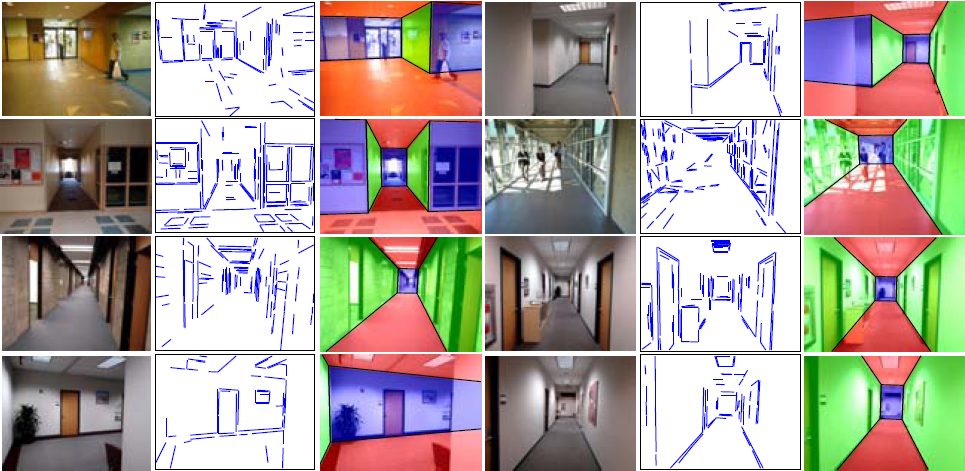
\includegraphics[width=\textwidth]{lee_result.png}
\caption{Inferred scene structure obtained for single images by Lee
  \etal \cite{Lee09}. Each triplet shows the original image, the
  detected line segments, and the final scene geometry.}
\label{fig:lee-result}
\end{figure}

\subsection{Texture Approaches}

Heitz and Koller \cite{Heitz08} have shown how to derive context from
texture structure present in images. Their ``Things And Stuff'' (TAS)
model relates the presence of objects (``things''), which have
specific boundaries, to the appearance of the nearby surfaces and
foliage (``stuff''), which have no crisp notion of spatial support.

Their approach is motivated by the observation that object positions
correlate with the appearance of their surroundings. For example, cars
and bikes are likely to appear near road--like patches, whereas
aeroplanes are likely to appear against a sky--like background.

They begin by running the normalised graph cuts algorithm of Ren and
Malik \cite{Ren03} to produce roughly homogeneous regions called
superpixels. Each such region is associated with a feature vector
comprising various colour and texture statistics, which, in their
model, is assumed to have arisen from a latent category variable, the
intention being that superpixels will be clustered into meaningful
groups like ``road'' and ``sky''. Meanwhile, a set of candidate object
detections is generated by invoking a standard object detector and
taking all detections above a certain threshold. The ``things'' are
related to the ``stuff'' by a set of observed variables representing
spatial relationships such as ``above'', ``beneath'', and ``next to''.

An advantage of the TAS model is that while object labels are required
for training, no explicit segmentations or labels are required for the
system to learn how to categorise the ``stuff'' regions since the
system is capable of learning these unsupervised. The authors achieve
this using the EM algorithm, which iterates between estimating the
superpixel labels and optimising the appearance parameters for each
label.

The authors also show how to learn a set of relationships that best
describe the dependencies between objects and their surroundings. This
involves augmenting the EM algorithm with a greedy search over
possible relationships, iteratively adding the best candidate out of a
pre--defined pool until convergence. This allows the system to adapt
to the most salient relationships for a specific problem, which will
differ between, say, images captured from satellites and the photos in
the VOC datasets \cite{VOC2009}. During evaluation both the object
labels and superpixel labels are unknown, so exact inference is
intractable. Instead, the authors use an approximate inference
technique called Gibbs sampling.  \figref{TAS-regions} shows some
example superpixel clusters along with their probabilistic
relationship to car detections.

\begin{figure}[htp]
\centering
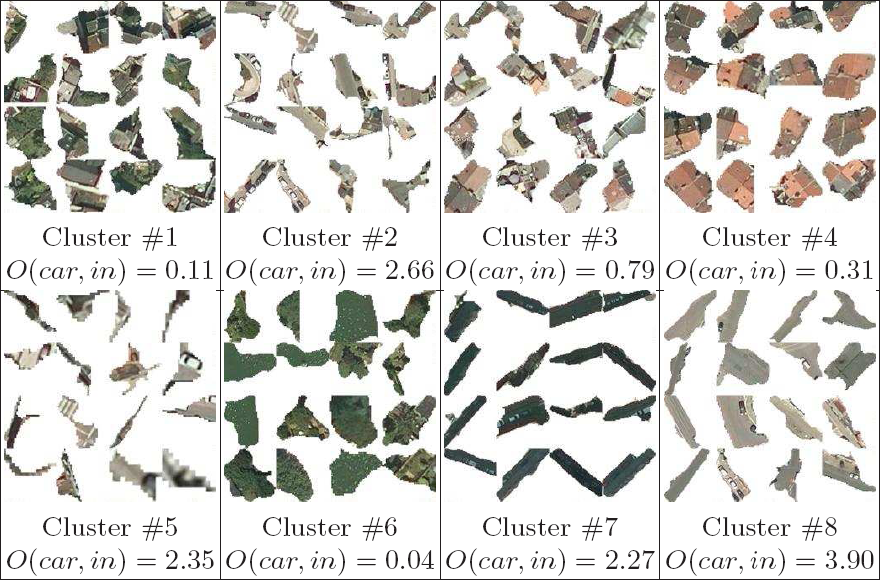
\includegraphics[width=0.75\textwidth]{TAS_regions.png}
\caption{Superpixels clusters generated by the TAS model of Heitz and
  Koller \cite{Heitz08}. Shown below each panel is the odds ratios for
  a car appearing near a superpixel from that class. The odds ratio is
  higher for road--like regions than for foliage-- or water--like
  regions.}
\label{fig:TAS-regions}
\end{figure}


\section{Conclusions}
Modern SLAM systems generate accurate metric maps of an environment,
and can do so robustly and efficiently using visual input alone
\cite{Klein07}. The higher--level problem of deriving semantic context
from such sensor data has been approached by several authors. Although
there is not yet a widely agreed--upon problem formulation, current
work in this area shows that semantics are important for many robotics
applications, and can be derived from a range of sensor
types. Important contributions include that of Martinez \cite{Mozos05}
and Stachniss \cite{Stachniss05}, who show that place categories can
be obtained from photometric and geometric cues, and Posner
\cite{Posner08}, who shows that scene regions can be associated with
semantic categories, again by combining vision and range sensors.

The contextual reasoning problem for single--image vision has received
comparatively greater attention. Torralba's seminal gist descriptor
\cite{Torralba03} has led to the development of many types of
contextual cues, including geometric \cite{Hoiem05,Saxena09}, textural
\cite{Heitz08}, and model--based \cite{Lee09} approaches. We are
encouraged by this work and hope to apply some of these approaches
within the robotics domain.
